\documentclass{article}
\usepackage{graphicx} % Required for inserting images
\usepackage{hyperref}
\usepackage[margin=3.5cm]{geometry}
\usepackage{subcaption}
\usepackage{float}
\usepackage{indentfirst}
\usepackage{amsmath}
\usepackage{amsmath, amssymb}

\usepackage{caption}
\DeclareCaptionFormat{myformat}{#1#2\textit{#3}}
\captionsetup{format=myformat, labelsep=endash}

\renewcommand{\contentsname}{Sommaire}

\title{PageRank - Rapport}
\author{Équipe GH13 \\ Vianney Hervy \& Louis-Clément Olivier}
\date{2023 - 2024}

\begin{document}

\maketitle
\newpage
% une page de garde avec titre, année, numéro d’équipe, membres de l’équipe, etc.

\tableofcontents

\newpage

\section{Introduction}

Dans ce projet nous avons implémenté un algorithme "PageRank" qui permet de classer des pages internet (ou n'importe quel ensemble de noeuds d'un graphe orienté) en fonction du nombre d'hyperliens qui y mènent depuis d'autres pages. L'algorithme ici utilisé a été conçu par Brin \& Page en 1998. Cet algorithme classe les pages internet par ordre décroissant de "popularité" en attribuant à chacune un poids entre $0$ et $1$. Plus une page est référencée par d'autres pages, plus elle est populaire. Plus les pages la référençant sont populaires, plus elle l'est. Ce calcul de poids est réalisé de manière itérative. À chaque itération, tous les poids sont mis à jour. On peut montrer que les poids convergent tous.

\section{Architecture}

L'application contient $4$ modules :
\begin{itemize}
    \item \texttt{PageRank\_Exceptions} qui définit les exceptions nécessaires au programme,
    \item \texttt{PageRank\_Doc} qui est responsable de l'affichage de la documentation,
    \item \texttt{Matrice\_Creuse} et \texttt{Matrice\_Pleine} (génériques) qui sont chacun responsables de la lecture et de l'interprétation des données de description du graphe et du calcul du PageRank dans la structure de donnée support associée
\end{itemize}

\noindent et $3$ programmes :
\begin{itemize}
    \item \texttt{PageRank} le programme principal qui gère les options de l'invite de commande et l'écriture des poids calculés dans le fichier de sortie,
    \item \texttt{Test\_Creuse} et \texttt{Test\_Pleine} les programmes de test respectifs des modules correspondants.
\end{itemize}

\begin{figure}[H]
    \centering
    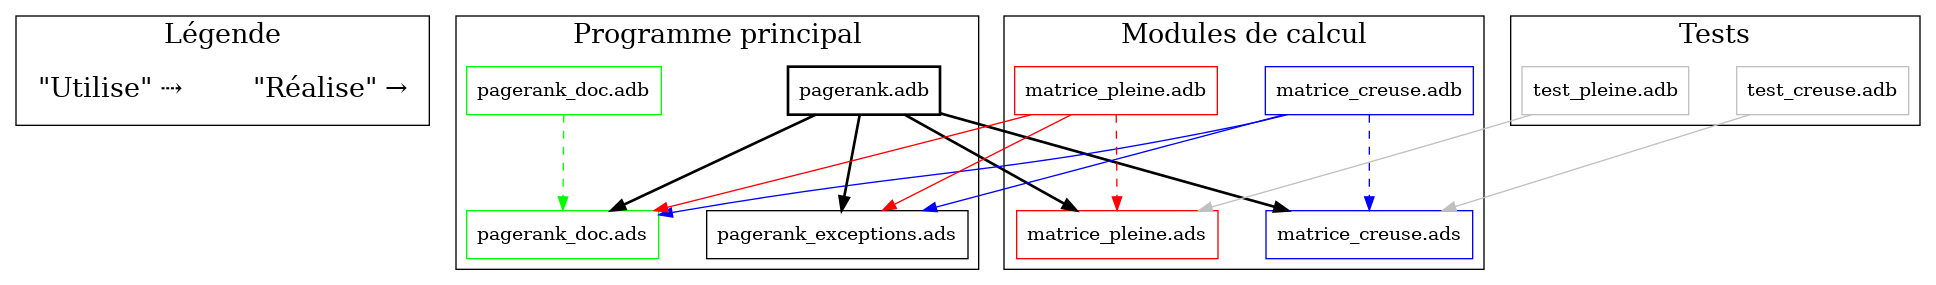
\includegraphics[width=\textwidth]{archi.png}
    \caption{Architecture de l'application PageRank}
\end{figure}

\noindent L'application utilise également les modules pré-définis suivants :
\begin{itemize}
    \item \texttt{Ada.Text\_IO} pour gérer les entrées/sorties textuelles (écriture/lecture), Il est également instancié pour lire et écrire des entiers,
    \item \texttt{Ada.Strings.Unbounded} pour manipuler des chaînes de caractères de taille inconnue,
    \item \texttt{Ada.Unchecked\_Deallocation} pour libérer l'espace alloué en mémoire à des pointeurs,
    \item \texttt{Ada.Command\_Line} pour lire les arguments entrés en ligne de commande.
\end{itemize}

\section{Détails de la réalisation des programmes}

\subsection{Programme principal \texttt{PageRank}}

Nous avons décidé d'inclure la quasi totalité du code dans les deux modules principaux.  \texttt{pagerank.adb} relie les différents composants de l'application. Il appelle les modules de calcul et de documentation en cas de besoin. Il ne contient que les procédures de gestion des arguments, de tri et d'écriture des poids.

\subsubsection{Instanciations}

Le programme principal utilise plusieurs modules génériques. Il instancie \texttt{Matrice\_Creuse} et \texttt{Matrice\_Pleine} avec le type \texttt{T\_Reel}, un type dont on peut facilement changer la définition dans le code : \texttt{Float}, \texttt{Long\_Float} ou encore un flottant avec la précision désirée.

Ce programme instancie aussi les modules \texttt{Ad.Text\_IO.Float\_IO} et \texttt{Ad.Text\_IO.Integer\_IO} avec respectivement les types \texttt{T\_Reel} et \texttt{Integer}. Ces modules permettront plus tard la lecture et l'écriture de nombres.

\subsubsection{Procédure \texttt{Tri\_Insertion}}

Cette procédure est appelée en fin d'exécution lorsque le vecteur poids final a été calculé. Elle trie les poids par ordre décroissant en gardant en mémoire le numéro associé au noeud. Pour cela, c'est l'algorithme de tri par insertion que nous avons choisi. Son fonctionnement est simple : on trie \texttt{V\_Trie} par insertion et à chacune des étapes où l'on échange deux valeurs, on échange également celles de \texttt{Ind\_Trie} qui contient les indices des noeuds.

\subsection{Module \texttt{PageRank\_Doc}}

Ce module, comme son nom l'indique, est responsable de la documentation. Il dispose de fonctions séparées pour afficher la documentation de chaque option possible en ligne de commande. Il dispose aussi d'exemples d'utilisation et d'un exemple de fichier graphe. En plus de cela, il permet l'affichage de toutes ces sections d'affilée lorsque l'utilisateur choisit l'option "-H" ou lorsqu'il ne met aucune option.

\subsection{Module \texttt{Matrice\_Creuse}}

Ce module implémente l'algorithme  en utilisant la structure de donnée "matrice creuse" décrite plus bas. Cette méthode est plus lente que la suivante mais utilise moins de mémoire (allocation dynamique de pointeurs). On peut choisir cette dernière en ajoutant l'option "-C" à la commande. C'est cette implémentation qui est choisie par défaut.

\subsubsection{Structures de donnée}

Le module \texttt{Matrice\_Creuse} n'utilise pas techniquement des matrices totalement creuses mais des matrices semis-creuses. Un vecteur creux consiste en une liste chaînée ou chaque case de la liste enregistre une valeur, l'indice de cette valeur  ainsi qu'un nouveau vecteur creux qui correspond au reste de la liste. cette représentation des vecteurs est très intéressante pour la complexité spatiale puisque toute les cases vides du vecteur ne sont pas enregistrée. on utilise pour les indices de ces vecteurs des \texttt{Integer} et pour les valeurs un type générique \texttt{T\_Reel} qui peut correspondre a tout les types de flottant (\texttt{Float}, \texttt{Long\_Float}...). Une matrice semi-creuse correspond a un tableau de vecteur creux, c'est a dire un \texttt{array} ou toute les cases sont des vecteur creux. Le vecteur plein peut être imaginé comme la première ligne de la matrice ou dans chaque case se trouve un vecteur creux en colonne. Cette implémentation simplifie fortement la fonction produit ce qui sera expliqué plus en détail dans la prochaine partie.

\subsubsection{Algorithmes}

Pour implémenter les vecteurs creux, nous avons réutilisé des fonctions déjà codé lors du TP sur les LCA, notamment la fonction \texttt{Modifier} qui permet d'ajouter un élément a un indice précis dans le vecteur creux. le module est aussi composé d'une fonction \texttt{Norme2Diff} qui calcule la norme au carré de la différence de 2 vecteurs ce qui est utile pour une des conditions d'arrêt de l'algorithme final.

La fonction produit (vecteur * matrice)  est particulière. En effet pour éviter que les matrices creuses perdent tout leur intérêt au moment de la construction de G (qui normalement remplit toute les cases), on n'ajoute pas $\frac{(1-\alpha)}{N}$ a toute les cases et on considère simplement que toute les cases vides (ie. qui n'existe pas dans la matrice creuse) valent en fait $\frac{(1-\alpha)}{N}$ pour les besoins du produit. cela permet de garder l'intérêt spatial des matrices creuses.

Une des grosses optimisations faite dans mon module pendant la dernière semaine de projet est d'arrêter d'utiliser une fonction qui prenait un indice et renvoyait la valeur du vecteur creux a cet indice. Cette méthode rendait mes codes très lent. Le bout de code qui divisait chaque élément par le nombre d'élément sur sa ligne par exemple avait une complexité temporelle en $O(N^4)$. J'ai donc modifié mon code pour que tout se fasse en un parcours de la matrice au lieu de recommencer un parcours a chaque fois que je veut chercher une valeur dans la matrice. cela permet de réduire des fonctions de $O(N^4)$ à $O(N^2)$

\subsubsection{Tests}

Le module est testé par le programme \texttt{teste\_pleine.adb}. Les fonctions purement calculatoires suivantes y sont testées : \texttt{Norme2Diff}, \texttt{Produit}, \texttt{Affine} (Produit Matrice*Scalaire).

\subsubsection{Structures de donnée}

Ce module implémente simplement une structure de donnée bidimensionnelle (\texttt{T\_Matrice}) et un tableau unidimensionnel (\texttt{T\_Vecteur}). Chacun de ces types est un \texttt{array} contenant des \texttt{T\_Reel}, type générique défini comme \texttt{digits} de précision réglable par l'utilisateur. \texttt{T\_Matrice} est utilisé pour modéliser les matrices (modifiées) d'adjacence. \texttt{T\_Vecteur} est utilisé pour stocker une donnée par noeud, par exemple le poids actuel (\texttt{Pi}), le rang du noeud dans le classement décroissant des poids (\texttt{Tri\_Vecteur\_Ind}) ou le nombre d'arcs sortant d'un noeud (\texttt{Nb\_Sortant}).

\subsubsection{Algorithmes}

Contrairement à son homologue \texttt{Matrice\_Creuse}, ce module n'a que très peu d'intérêt algorithmiquement. Chaque fonction de calcul est une double boucle POUR qui remplie case par case la \texttt{T\_Matrice} ou le \texttt{T\_Vecteur} en sortie. La seule spécificité pertinente est l'implémentation d'un second mode de calcul du vecteur des poids dans le cas où $\varepsilon = 0.0$. Dans ce cas là, on sait qu'exactement $K$ itérations seront effectuées avant de renvoyer $\pi_k$. Or, on a $\pi_{k+1} = \pi_k * G$ donc $\pi_K = \pi_0 * G^K$. En calculant $G^K$ séparément, on ne gagnerait pas particulièrement de temps, mais si on fait usage de l'exponentiation rapide, là, on gagne en complexité. Elle décrit un algorithme récursif comme tel :
$$G^K =
    \left\{\begin{array}{cl}
        I_N                   & \text{ si } K = 0                \\
        (G^2)^\frac{K}{2}     & \text{ si } K \text{ est pair}   \\
        G*(G^2)^\frac{K-1}{2} & \text{ si } K \text{ est impair}
    \end{array}\right.$$
Toutefois, cette structure de donnée prend beaucoup de place et donc la limitation première n'est pas le temps d'exécution mais bien la mémoire utilisée.

\subsubsection{Tests}

Le module est testé par le programme \texttt{teste\_pleine.adb}. Les fonctions purement calculatoires suivantes y sont testées : \texttt{Norme2}, \texttt{"-"}, \texttt{"+"}, \texttt{"*"} (produit matriciel entre matrices carrées), \texttt{Exponentiation\_rapide} (procédure récursive), \texttt{"*"} (produit scalaire/matrice , \texttt{"*"} (produit vecteur/matrice). Il contient également une procédure de test pour la procédure d'extraction \texttt{Extraire\_Arc}.

\subsection{\texttt{Text\_IO}}

Une particularité de ce projet (par rapport aux précédents de PIM) est la lecture/écriture de texte. Elle intervient dans la récupération des options en ligne de commande, dans l'extraction du graphe du fichier d'entrée et dans l'écriture de la sortie.

\subsubsection{Lecture du fichier graphe (\texttt{.net})}

La lecture du fichier graphe se fait en deux temps : la lecture de la première ligne (nombre de noeuds) par \texttt{pagerank.adb} puis la lecture des lignes suivantes (arcs) par les modules de calcul.

La première étape vérifie l'existence (resp. la non-vacuité) du fichier graphe sinon lève \texttt{Fichier\_Introuvable\_Exception} (resp. \texttt{Fichier\_Vide\_Exception}). Ces deux exceptions ne sont pas traitées dans les ouvertures suivantes du fichier, on suppose que l'on ne s'est pas amusé à supprimer ou modifier ce dernier entre les deux ouvertures.

La deuxième étape a lieu dans la fonction \texttt{Extraire} qui itère sur les lignes du fichier en stockant chacune dans une \texttt{Unbounded\_String}. Cette ligne est ensuite passée à la procédure \texttt{Extraire\_Arc} qui, à l'aide de deux \texttt{Get}, récupère les deux sommets de l'arc correspondant. La matrice $H$ est alors peu à peu construite.

\subsubsection{Autres}

La procédure \texttt{Get\_Args} de \texttt{pagerank.adb} lit argument après argument dans une boucle TANT QUE jusqu'à l'avant dernier où il le lit comme un nom de fichier. À chaque argument, une structure SELON fait correspondre l'action associée.

Pour ce qui est le est de nouveau \texttt{pagerank.adb} qui la réalise. Ce sont deux boucles POUR qui itèrent sur les vecteurs pour les écrire dans les fichiers correspondants.

\subsection{Gestion des exceptions et module \texttt{PageRank\_Exceptions}}

L'application est codée suivant les principes de la programmation défensive. Dans le cas où une exception est atteinte, elle est soit traitée, soit levée et renvoyée à l'utilisateur avec un message expliquant où est l'erreur et une section de la documentation indiquant la bonne marche à suivre.

Les $4$ exceptions définies sont les suivantes :
\begin{itemize}
    \item \texttt{Arg\_Option\_Exception} levée lorsque les arguments en ligne de commande sont mal formulés (argument inconnu ou valeur incorrecte). Lors de la récupération des arguments dans \texttt{pagerank.adb} par \texttt{Get\_Args}, elle peut-être levée suivie de l'argument incorrect.

    \item \texttt{Fichier\_Introuvable\_Exception} levée lorsque le fichier graphe d'entrée n'est trouvé à l'adresse indiquée. Elle n'est traitée que lors de la première ouverture dans \texttt{pagerank.adb}, on suppose que l'on ne s'est pas amusé à supprimer le fichier dans le court instant qui sépare les deux ouvertures.

    \item \texttt{Fichier\_Format\_Exception} levée lorsque le texte dans le fichier graphe ne correspond pas au format défini dans le sujet. C'est à dire qu'il n'y a pas exactement un entier strictement positif sur la première ligne ou que les suivantes ne contiennent pas exactement 2 entiers positifs inférieurs strictement au premier et séparés d'un espace. Cette exception peut être levée par \texttt{Extraire\_Arc} dans les modules \texttt{Matrice\_Pleine} et \texttt{Matrice\_Creuse}.

    \item \texttt{Fichier\_Vide\_Exception} levée lorsque le fichier graphe est vide. Elle peut être levée par \texttt{pagerank.adb} lors de la première ouverture du fichier.

    \item \texttt{Afficher\_Doc\_Exception} levée lorsque l'utilisateur demande d'afficher l'aide, elle n'est utilisée que pour stopper le programme et afficher la documentation. Elle peut être levée dans \texttt{pagerank.adb} par \texttt{Get\_Args} quand l'option "-H" est lue.
\end{itemize}
% l’explication de la manière dont le programme et les modules ont été mis au point

% 2 modules

\section{Résultats}

\begin{center}
    \begin{tabular}{|c|c|c|c|c|}
        \hline
        Implémentation \textbackslash\ graphe & Exemple & Worm   & Brainlinks    & Linux26       \\
        \hline
        Matrice Creuse                        & 0.06s   & 0.016s & 10.83s        & 2min50s       \\
        \hline
        Matrice Pleine                        & 0.010s  & 1.59s  & $\varnothing$ & $\varnothing$ \\
        \hline
    \end{tabular}
\end{center}

Le code en $O(N^2)$ ne permettent pas de faire tourner le code sur le graphe Linux26 de façon satisfaisante même en utilisant des matrices creuses, puisque une seule itération de la fonction produit prend en moyenne 3min45. avec le module matrice pleine, les graphes Brainlinks et Linux26 provoque des \texttt{Storage\_Error} qui empêche de run le programme.


% les durées d’exécution du programme en fonction des implantations (pleine et creuse), sur les exemples fournis et une analyse des résultats constatés

\section{Difficultés rencontrées}

La première difficulté s'est présentée lors de l'extraction des données du graphe du fichier d'entrée. Pour déclarer la matrice (creuse ou pleine), il nous fallait déjà le nombre de noeuds du graphe. La solution que nous avons trouvé est d'ouvrir le fichier et de lire ce nombre en amont du calcul du PageRank, dans le programme principal. Puis de le rouvrir, ignorer la première ligne et ensuite récupérer tous les arcs.

La principale difficulté est apparue à la fin de la réalisation du projet. Lorsque l'on a essayé de faire tourner le sujet \texttt{linux26.net} en implémentation matrice creuse, l'exception \texttt{STORAGE\_ERROR} a été levée. La déclaration simultanée de plus d'une matrice creuse et deux vecteurs pleins de taille $285510$ n'est pas acceptée. Pour contourner ce problème, nous avons dû créer des fonctions intermédiaires de sorte que les portées des larges objets déclarés ne se chevauchent pas. Cette limitation n'est pas présente sur nos PC respectifs, seulement sur les machines de l'école.

Plus tard, nous avons compris qu'il était possible de faire tourner jusqu'à \texttt{worm.net} avec l'implémentation matrice pleine. Pour optimiser la mémoire, nous avons cette fois remplé toutes les fonctions de calcul par des procédures. Certaines variables comme \texttt{Temp} dans \texttt{Calcul\_Plein} sont utilisées dans différents contextes sans rapport. Cette technique permet de ne pas déclarer plusieurs variables (qui prendront donc plus de place). Une autre solution possible était de partitionner ces programmes en sous-programmes afin de réduire la portée (donc la durée de l'occupation en mémoire) de ces variables.

% les difficultés rencontrées et les solutions adoptées en justifiant vos choix (en particulier quand vous avez envisagé plusieurs solutions)

\section{Grilles d'évaluation}

% les grilles d’évaluation des raffinages et du code complétées (cf Moodle)
\vspace{2em}
\hspace{-1cm}
\begin{center}
    \begin{tabular}{|p{11cm}|p{1cm}|p{1cm}|}
        \hline
                                                                                                                                                 & LCO & VH \\

        \hline
        \texttt{Respect de la syntaxe} Ri: Comment "... une action complexe ..." des actions combinées avec des structures de contrôle ? Rj: ... & +   & A  \\
        \hline
        \texttt{Verbe à l'infinitif pour les actions complexes}                                                                                  & +   & +  \\
        \hline
        \texttt{Nom ou équivalent pour expressions complexes}                                                                                    & +   & +  \\
        \hline
        \texttt{Tous les Ri sont écrits contre la marge et espacés}                                                                              & +   & +  \\
        \hline
        \texttt{Les flots de données sont définis}                                                                                               & +   & +  \\
        \hline
        \texttt{Une seule décision ou répétition par raffinage}                                                                                  & A   & A  \\
        \hline
        \texttt{Pas trop d'actions dans un raffinage (moins de 6)}                                                                               & A   & +  \\
        \hline
        \texttt{Bonne présentation des structures de contrôle}                                                                                   & +   & A  \\
        \hline
        \texttt{Le vocabulaire est précis}                                                                                                       & +   & +  \\
        \hline
        \texttt{Le raffinage d'une action décrit complètement cette action}                                                                      & A   & A  \\
        \hline
        \texttt{Le raffinage d'une action ne décrit que cette action}                                                                            & A   & +  \\
        \hline
        \texttt{Les flots de données sont cohérents}                                                                                             & +   & +  \\
        \hline
        \texttt{Pas de structure de contrôle déguisée}                                                                                           & +   & +  \\
        \hline
        \texttt{Qualité des actions complexes}                                                                                                   & +   & +  \\
        \hline
    \end{tabular}
\end{center}


\section{Répartition du travail}

\begin{center}
    \begin{tabular}{|c|c|c|c|c|}
        \hline
        Programme/activité       & Spécifier & Programmer & Tester & Relire \\
        \hline
        \texttt{Matrice\_Creuse} & LCO       & LCO        & LCO/VH & VH     \\
        \hline
        \texttt{Matrice\_Pleine} & VH        & VH         & VH/LCO & LCO    \\
        \hline
        \texttt{Pagerank}        & VH        & VH         & VH     & LCO    \\
        \hline
    \end{tabular}
\end{center}


\end{document}